% Section content template for individual Educative lessons
% This file contains the actual content for a specific section
% Generated from Educative API section content

% Section: Requirements for the Vending Machine
% Section ID: 6161581157384192
% Section Slug: requirements-for-the-vending-machine
% Generated: 2025-12-11T20:25:35.333479

This lesson outlines the functional and operational requirements for the Vending Machine system. Identifying and understanding requirements is essential to defining the system's scope and ensuring a robust, user-friendly design.
\\
We'll use the notational convention to identify each requirement with a unique label ``Rn,'' where ``R'' is short for requirement and ``n'' is a natural number.

\subsection{Requirement collection}\label{M1zVrNdE_9LN4LFQUVYNN}
\\
The requirements for the vending machine problem are defined below:

% \vspace{-1.0\baselineskip}
\noindent
\begin{minipage}[t]{0.48\textwidth}\vspace{0pt}
\begin{itemize}
\item
\textbf{R1:}~The vending machine stores and manages different types of products, each placed at a unique slot within the machine.
\item
\textbf{R2:}~The vending machine can be in one of these three states:

\begin{itemize}
\item
\textbf{NoMoneyInsertedState:} There is no money inserted into the machine.
\item
\textbf{MoneyInsertedState:} Money is inserted into the machine.
\item
\textbf{DispenseState:} The machine gives out the product.
\end{itemize}
\item
\textbf{R3:}~The system has two primary actors: the customer and the operator.
\item
\textbf{R4:}~The admin can add or remove new products to the machine.
\end{itemize}
\end{minipage}
\hfill
\begin{minipage}[t]{0.48\textwidth}\vspace{0pt}
\centering
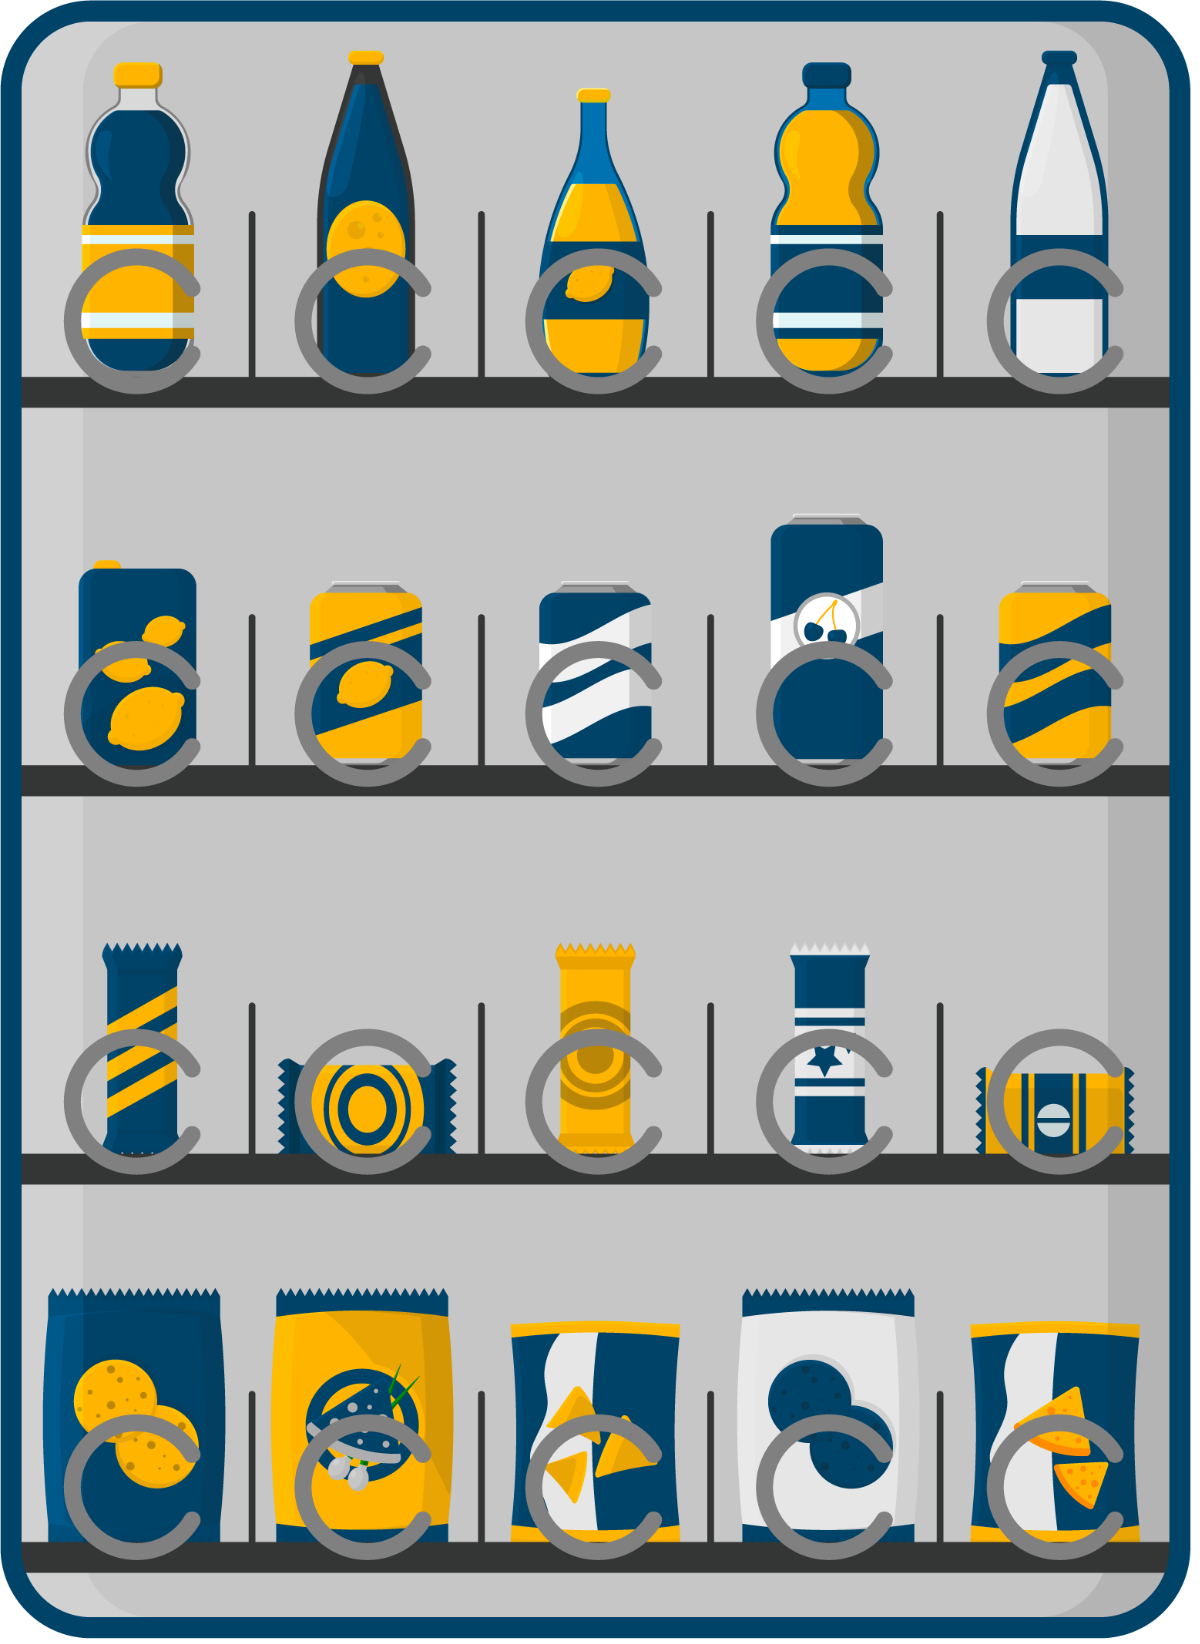
\includegraphics[width=0.5\textwidth]{Images/chapter_11/section_6161581157384192/4728542833410048.png}
\end{minipage}

% \vspace{-1.0\baselineskip}
\noindent
\begin{minipage}[t]{0.48\textwidth}\vspace{0pt}
\begin{itemize}
\item
\textbf{R5:}~The system should allow the users to select a product they want to purchase from the machine by specifying the rack number.
\item
\textbf{R6:}~Users can insert money (cash) into the machine.
\item
\textbf{R7:}~The system should be able to calculate the money inserted into the machine.
\end{itemize}
\end{minipage}
\hfill
\begin{minipage}[t]{0.48\textwidth}\vspace{0pt}
\centering
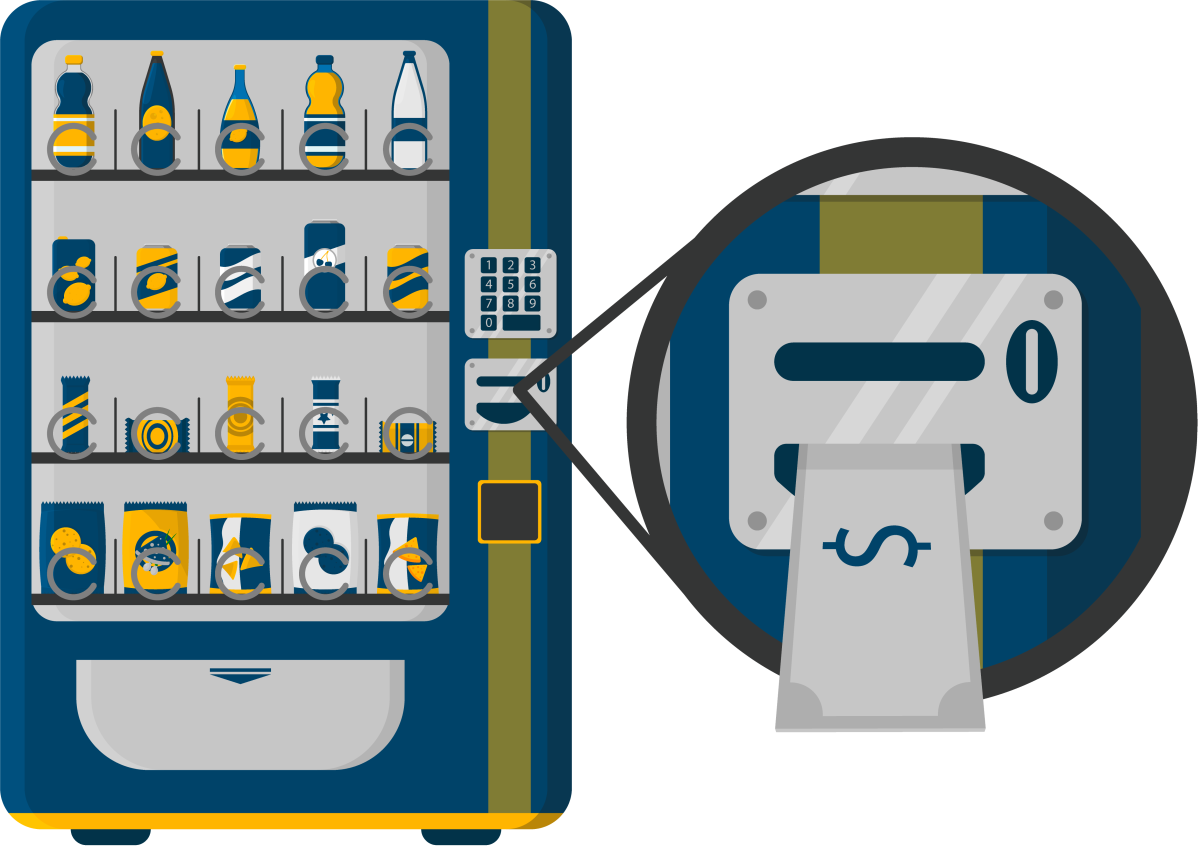
\includegraphics[width=0.5\textwidth]{Images/chapter_11/section_6161581157384192/4828243897352192.png}
\end{minipage}

% \vspace{-1.0\baselineskip}
\noindent
\begin{minipage}[t]{0.48\textwidth}\vspace{0pt}
\begin{itemize}
\item
\textbf{R8:}~The system should check whether the user inserted the exact amount required for the specific product into the machine.
\item
\textbf{R9:}~If the amount exceeds the product price, the system should change the user back and dispense the product.
\item
\textbf{R10:}~If the amount exceeds the product price, the system should display an error message and return the money.
\end{itemize}
\end{minipage}
\hfill
\begin{minipage}[t]{0.48\textwidth}\vspace{0pt}
\centering
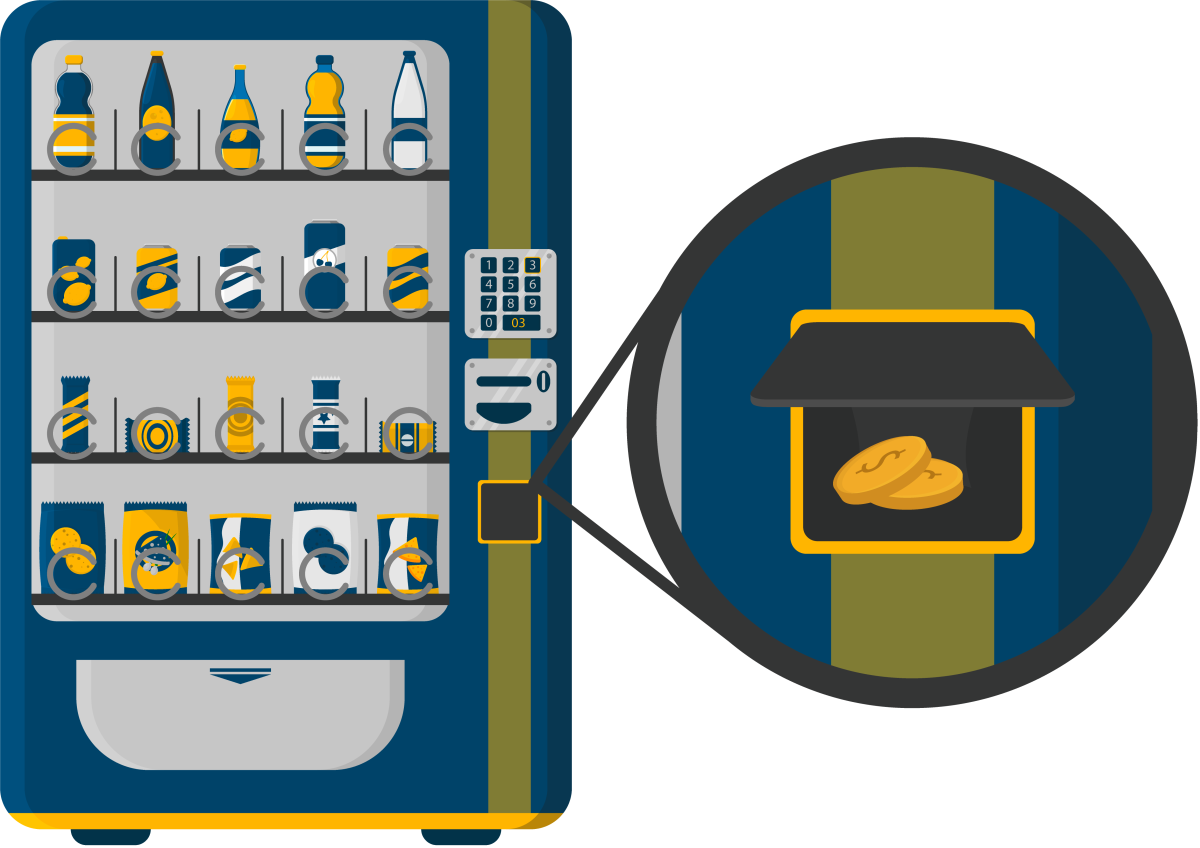
\includegraphics[width=0.5\textwidth]{Images/chapter_11/section_6161581157384192/4549930922541056.png}
\end{minipage}

We've identified our requirements for the problem, and in the next lesson, we will define the class diagram of our vending machine system.

% End of section content